% ##################################################################################################################
\chapter{Hamburg Wilhelmsburg}
\label{ch:hhw}
\hfill \textbf{Authors:} Hubert Klüpfel, Gregor Lämmel

\editdone{This text has undergone the professional edit. Please no grammatical changes anymore! They are most-probably wrong.}

% ##################################################################################################################
Hamburg-Wilhelmsburg's evacuation was described as a case study; the scenario was created using \gls{matsim}'s \gls{grips} \gls{extension}. Technical details of this extension are given in Chapter~\ref{ch:evacuation}. 

Wilhelmsburg was severely flooded in 1962; since then, many structural and operational improvements have been implemented. At the time of the flood, the housing situation was precarious, with many people still living in provisional housing built after World War II damage. In additional to  construction of much more stable buildings, precautions against flooding have been taken and sea and flood walls have been heightened. However, evacuation can still be necessary under certain circumstances. The relocation of one of the major Wilhelmsburg roads, the B75, also influences any evacuation traffic, since it is one of the major north-south arteries. In this case study, road relocation consequences on the evacuation of Hamburg-Wilhelmsburg were investigated.

% ==================================================================================
\section{Brief Description}
The scenario investigated here was the relocation of highway B75 in Wilhelmsburg. Two cases were investigated, as summarized in the following table.
%
\createtable%
	{Scenarios}%
	{Scenarios}%
	{\label{table:b75scenarios}}%
	{%
	\begin{tabular}{|l | l|}
	\hline
	1 & Current location of B75 with restricted directional choice\\
	2 & New location of B75 with restricted locational choice\\
	\hline
\end{tabular}
}%
{}%
%
\createfigure%
	{New and old section of B75}%
	{The current trail of highway B75 is shown in the center of the image. The new trail is east of it close to the railroad.}%
	{\label{fig:overviewB75}}%
	{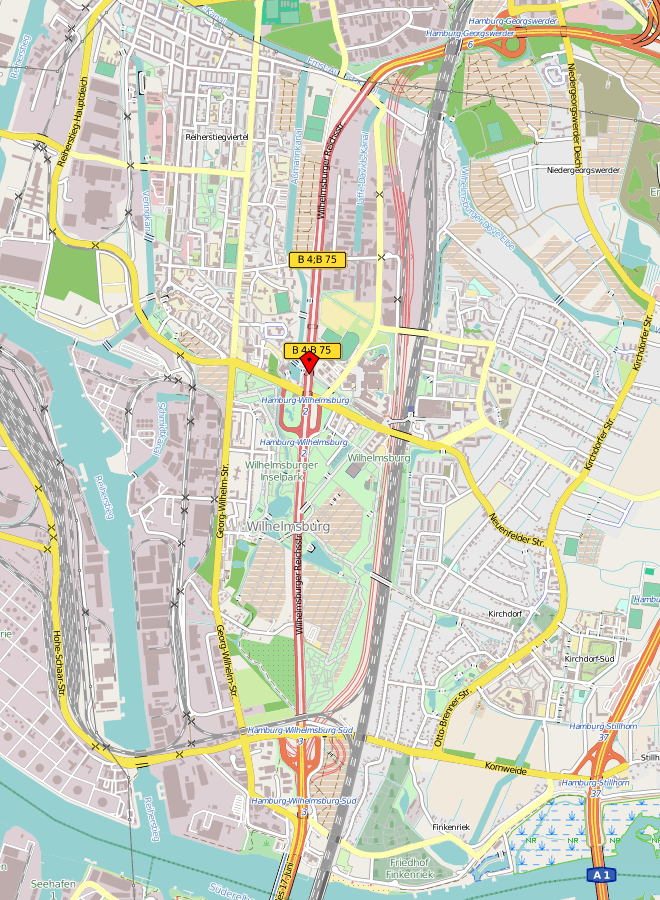
\includegraphics[width=0.7\linewidth]{using/figures/B75overview}}%
{}
%
The investigation highlighted differences in the evacuation traffic for both variants of the B75 trail. As seen in Figure~\ref{fig:overviewB75}, the new trail ``B75 new'' was located generally next to the existing railway track. In the south, the new variant was connected to the existing highway at the junction ``Hamburg Wilhelmsburg Süd'' (just north of the bridge across the river Elbe); in the north, it was connected to the existing highway just before the junction ``Hamburg Georgswerder''. The main differences between the two variants were access routes to highway B75 in the center of Wilhelmsburg.

% ==================================================================================
\section{Road Network}
The \gls{matsim} road network was generated (``imported'') from the Hamburg \gls{osm} file. This file was downloaded from \url{www.geofabrik.de}. Fortunately, the \gls{osm} file already contained the new B75 highway track, marked by an attributed ``open 2016''. Therefore, the two networks for the ``B75 old'' and ``B75 new''  variants could be derived from the same \gls{osm} file. For the variant ``B75 old'', this file could be directly imported. For the variant ``B75 new'', the section of B75 to be relocated was removed in a first step. In a second step, the new B75 track was connected to the existing road network, \ie the B75 north at junction ``Georgswerder'' in the north and junction ``Hamburg Wilhelmsburg Süd'' in the south.

Additionally, the internal on and off-ramps to the B75 were added. The two variants of the resulting road network, \ie ``B75 old'' and ``B75 new'' are shown in Figure~\ref{fig:b75oldnew}.
%
\createfigure%
{Comparison between network for the old and new track of the B75.}%
{Comparison between network for the old and new track of the B75.}%
{\label{fig:b75oldnew}}%
{%
  \createsubfigure%
  {}%
  {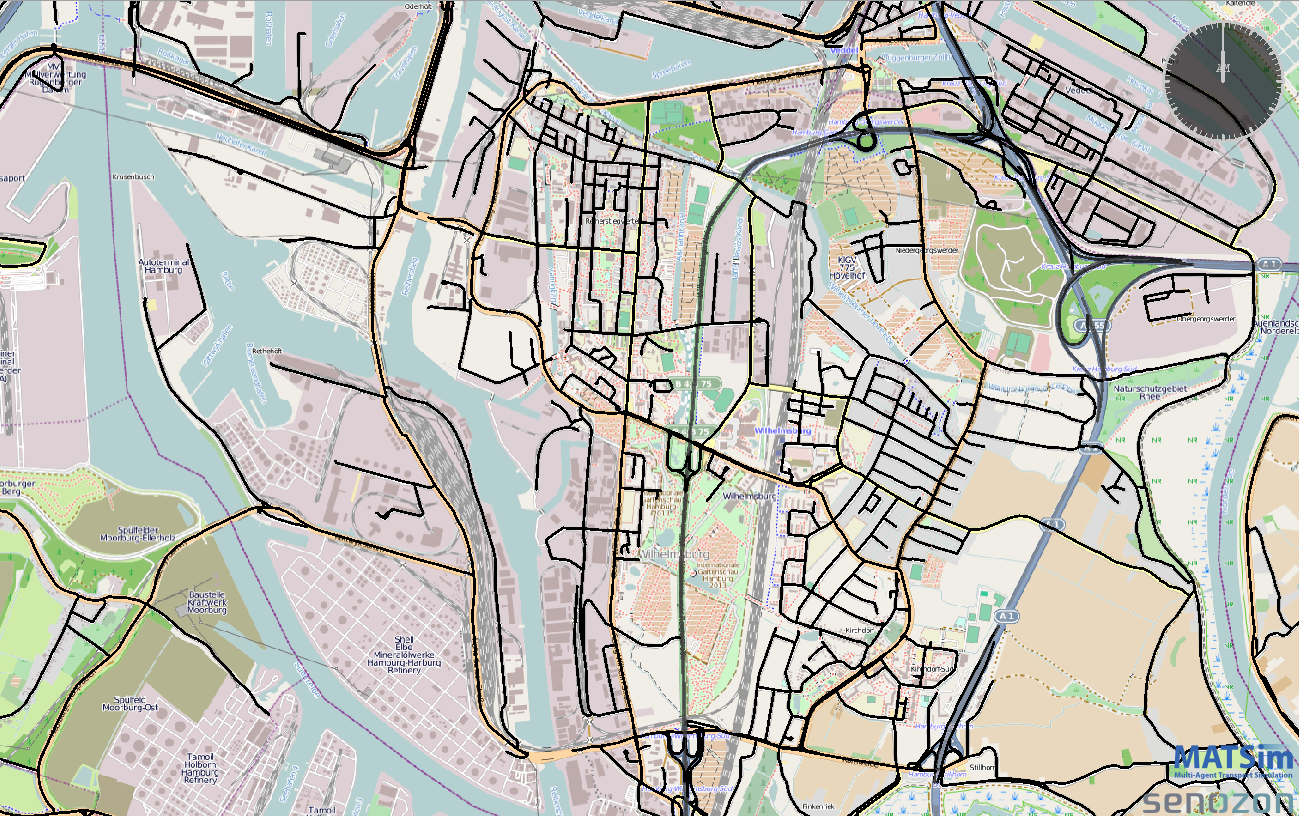
\includegraphics[width=.475\linewidth]{using/figures/B75old}}%
  {}%
  {}%
  \createsubfigure%
  {}%
  {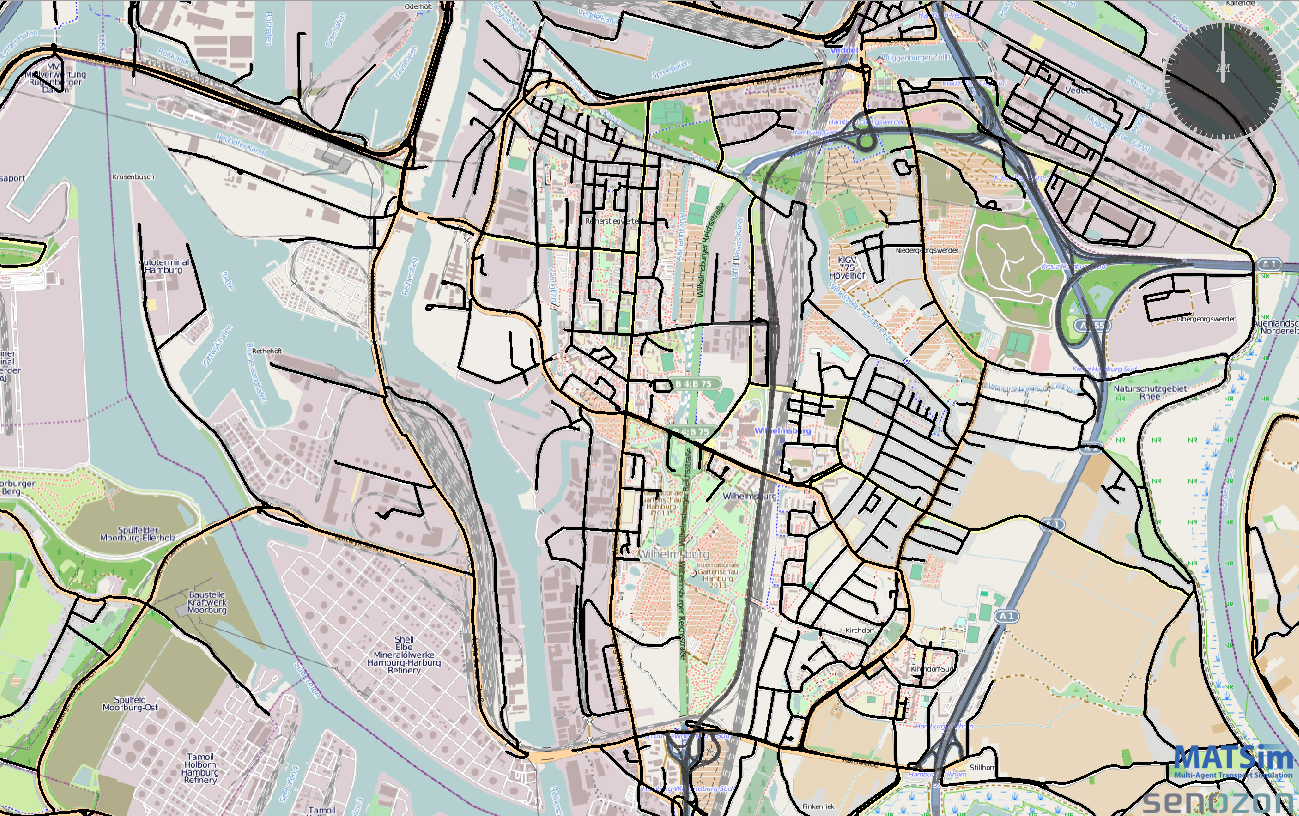
\includegraphics[width=.475\linewidth]{using/figures/B75new}}
  {}%
  {}% 
}%
  {}%

In an evacuation, some roads would be blocked to avoid intersecting traffic and inbound traffic would be blocked. The following streets were thus deleted in the \gls{osm} file:
%
\begin{compactitem}
	\item Neuenfelder Str. 
	\item Im Schönenfelde
	\item Elsterweide
	\item Kirchdorfer Str.
\end{compactitem}
%
This was illustrated in Figure~\ref{fig:b75sperrung}.
%
%
\createfigure%
{Closed roads in Hamburg-Wilhelmsburg}%
{Roads closed during evacuation}%
{\label{fig:b75sperrung}}%
{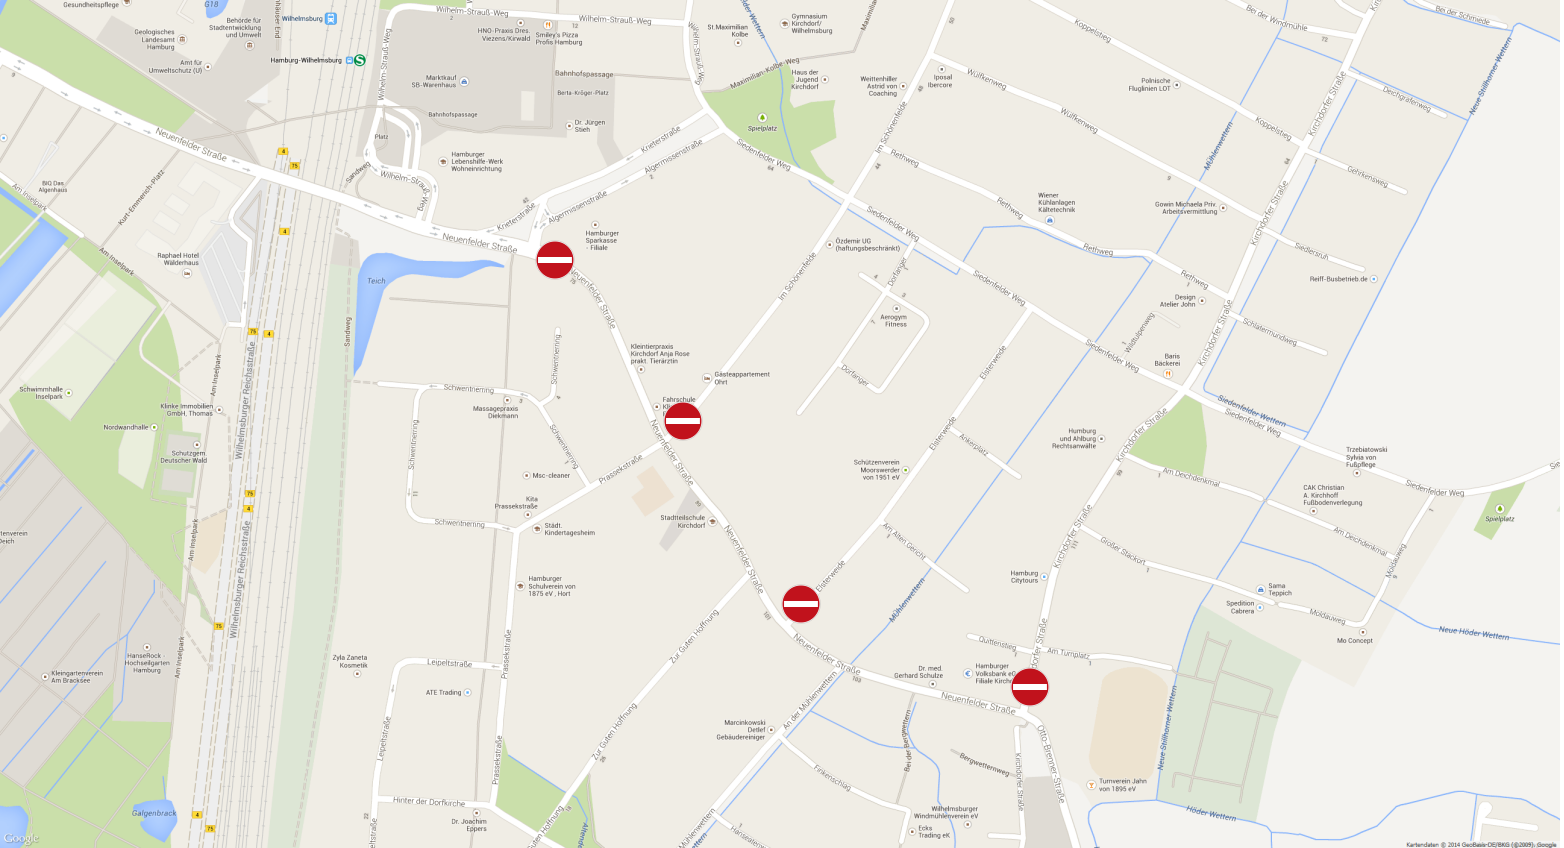
\includegraphics[width=0.7\linewidth]{using/figures/B75sperrung}}%
{}

% ==================================================================================
\section{Evacuation Scenario}
The comparison of the two variants was based on overall evacuation time, clearing time of different cells (squares in the area that had to be evacuated) and the number of cars using the road network (utilization).

As described in Chapter~\ref{evac:section:fifteenminute}, the input files for the network (\gls{osm}), the area (shp), and the population (shp), as well as the parameters for sample size and departure time distribution, were specified and assessed via a \gls{gui}. They were stored in an \gls{xml} file. The scenario \gls{xml} file for the existing (or ``old'', in German ``alt'') track of highway B75 was shown in the following listing. 

\lstinputlisting[language=XML]{using/scenarios/whb_B75alt.xml}

% ==================================================================================
\subsection{Departure Time Distribution}
The departure time distribution was specified in the file \lstinline|scenario.xml|. The values were in seconds, \ie a normal distribution with a mean value (mu) and a standard deviation (sigma) of 30\,minutes in the range of zero (earliest) to one hour (latest) was chosen. 
More details about time distributions were discussed in Chapter~\ref{chap:evac:eq:mu}. This distribution reflected certain assumptions made about evacuation procedure. The overall time frame, based on the warning time, was minimum 7\,hours. The preparation phase took three hours, setting up the buses and alarming the emergency staff twp hours and boarding of the buses was estimated at one hour. Available time for the evacuation was three hours, with a one-hour buffer. 
The warning via radio was started at t=0\,hours and local warning (\eg by police cars, sirens, and via short messages) at t=1\,hours; simulation reference point was set to t=3\,hours. The overall time acceptance criterion for the simulation was the required safe evacuation time (for simulation by car) of less than three hours (including reaction time). The reaction time set in the simulation could therefore be interpreted as decision-making time after readying personal belongings. In short: \gls{aset} determined by flooding was 3\,hours and the \gls{rset} was determined by the simulation. The criterion for a successful evacuation was \gls{aset} $>$ \gls{rset}.

% ==================================================================================
\subsection{Population Size}
As explained previously, population was not stored in the scenario file, but in the population shape file, possibly consisting of several polygons. Number of persons was stored as an attribute for each polygon. Here, one must assume that only part of the population would have to evacuate; for many, escape to higher ground might be sufficient. Detailed information on the different procedures can be found at \url{http://www.hamburg.de/sturmflut/3425646/sturmflut-download-1/} (in German).

Each agent represented one evacuee traveling by car. To independently check the number of agents based on the simulation files, one could open the file \lstinline|population.dbf| with a database or spreadsheet editor. Note that the number specified in the \lstinline|population.shp| (resp. \lstinline|population.dbf|) was multiplied with the \lstinline|sampleSize| when converting the files to \gls{matsim} input, \ie in this case, the \lstinline|population.xml.gz| located in the output directory.

The population was initially distributed as shown in Figure~\ref{fig:B75initial}. 
%
\createfigure%
{Initial distribution of agents.}%
{The initial distribution of the agents for the evacuation of Wilhelmsburg (for both cases, B75 new and old).}%
{\label{fig:B75initial}}%
{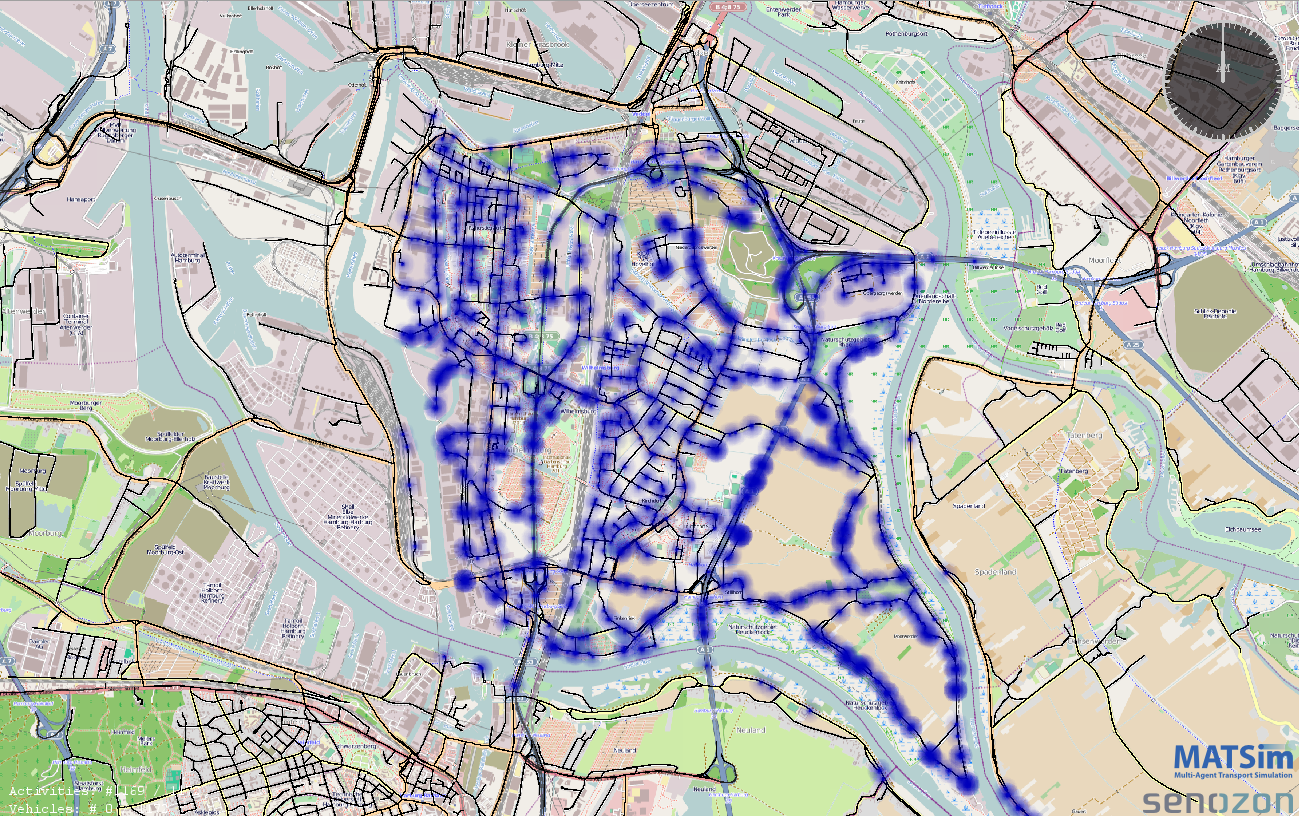
\includegraphics[width=0.7\linewidth]{using/figures/B75initial}}%
{}
The algorithm that converted the area and population (\ie \lstinline|area.shp| and \lstinline|population.shp|) was described in Chapter~\ref{chap:evac:fig:area_pop}). It assigned agents to the edges of the network. In the case study, harbor areas were left out and agents were equally distributed to streets in the housing (and agricultural) areas of Wilhelmsburg (Figure~\ref{fig:B75initial}).
Of course, this could have been further refined by going to a block, or even house level and assigning the population according to detailed statistical housing data. This was not undertaken for this simulation, for two reasons. First, many assumptions were made about behavior, initial location, and share of population that had to evacuate. Therefore, the level of detail seemed to be sufficient. Second, each agent represented a car driver, \ie in the simulation, all cars registered in Wilhelmsburg left the area. Considering that inbound, as well as through traffic would be prohibited when flooding level exceeded a certain threshold, this was a ``worst case'' assumption resulting in a heavy traffic load. To summarize, the overall approach was justified to assess highway B75 relocation based on heavy traffic load with a reaction time span between 0 and 1\,hour.

% ==================================================================================
\section{Simulation Results}
The simulation results are summarized in Table~\ref{table:b75results}. The 0th iteration is based on shortest distance only. 
%
\createtable%
{Results.}%
{Results.}%\begin{table}[!ht]
%	\centering
%	\caption{Results.}
{\label{table:b75results}}%
{%
\begin{tabular}{|c|c|c|}
	\hline \rule[-2ex]{0pt}{5.5ex}  & B75 old & B75 new \\ 
	\hline \rule[-2ex]{0pt}{5.5ex}  Iteration & Time &  (hh:mm) \\ 
	\hline \rule[-2ex]{0pt}{5.5ex}  00 & 04:45 &  05:00\\ 
	\hline \rule[-2ex]{0pt}{5.5ex}  10 & 01:52 &  01:58\\ 
	\hline \rule[-2ex]{0pt}{5.5ex}  20 & 01:42 &  01:46\\ 
	\hline \rule[-2ex]{0pt}{5.5ex}  30 & 01:40 &  01:42\\ 
	\hline 
\end{tabular}
}%
{}% 
%
This might have resulted in ``strange'' behavior, as illustrated in the following Figure~\ref{fig:B75iteration0} (south of the bridge across the Elbe river, near the junction ``Gro{\ss}moordamm''). The road network had a circular shape; it was cut out from the osm road network according to the \lstinline|area.shp|, which was, in our case, just a circle. Since all the agents were taking the shortest path in iteration~0, they headed to the nearest road out of the evacuation area. Technically, the boundary links in the network were connected to a super link when creating the \gls{matsim} network from the \gls{osm} file and the \lstinline|area.shp|. This super-link was the destination in all evacuees' plans. 
%
\createfigure%
{Results for B75 old, iteration 0}%
{Results for B75 old, iteration 0.}%
{\label{fig:B75iteration0}}%
{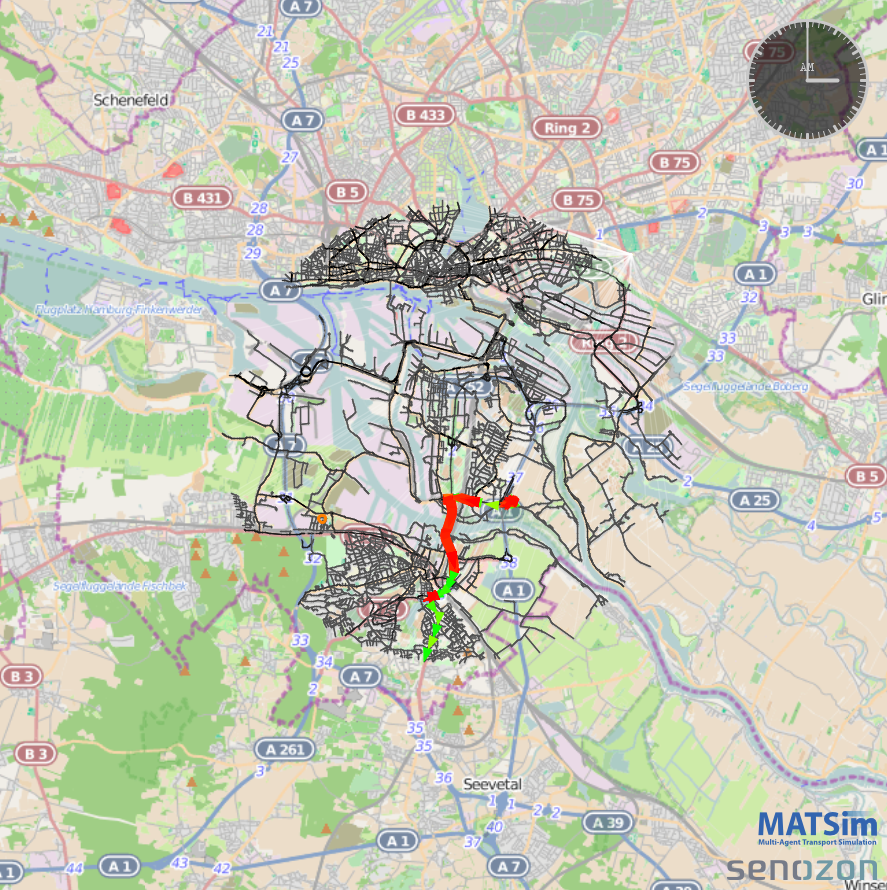
\includegraphics[width=0.7\linewidth]{using/figures/B75iteration0}}%
{}
%
A second factor that contributed to congestion in iteration~0 was a short cut via an on- and off-ramp of Autobahn A253 at ``Gro{\ss}moordamm''. Capacity of the on- and off-ramp was 1\,500 cars per hour, compared to 4\,000 cars per hour on the highway. Thus, the short cut (which was shorter in distance, the reason agents chose it) was a bottleneck, resulting in artificial congestion in iteration~0.
Therefore, the 0th iteration was unsuitable for assessing the overall evacuation time. As can be seen from Table~\ref{table:b75results} above, for both cases, from iteration~10 on, time presumably converges to some realistic value. This was also illustrated in Figure~\ref{fig:B75iteration20} where the situation at t=1:30\,hours was shown for iteration~20.
%
\createfigure%
{Results for B75 old, iteration~20}%
{Results for B75 old, iteration~20.}%
{\label{fig:B75iteration20}}%
{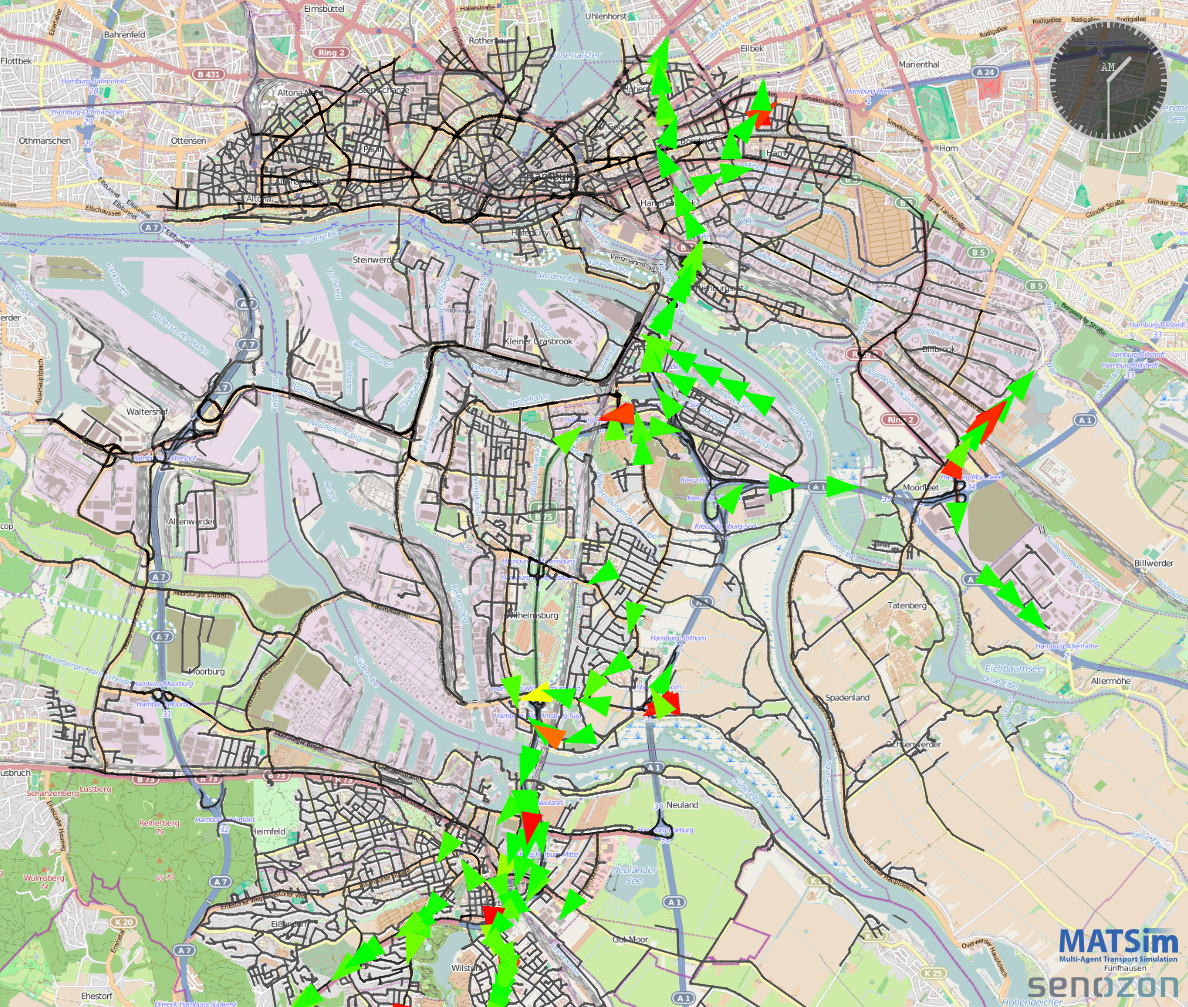
\includegraphics[width=0.7\linewidth]{using/figures/B75iteration20}}%
{}

In summary, relocation of highway B75 had no major influence on the overall evacuation time. The evacuation time of about two hours was also within the available safe egress time, as described in the previous section. 

It would certainly have been possible to analyze the results further. The two screenshots above, for the situation in iteration 0 at t=3\,hours and for iteration 20 at t=1.5\,hours, were created with \gls{senozon} Via (the visualizer presented in Chapter~\ref{ch:via}). As a conclusion to this chapter and an illustration for the built-in capabilities of \gls{grips} for analyzing simulation results, road utilizations of the two variants are shown in Figure~\ref{fig:b75utilization}.
%
\createfigure%
{Network utiliziation for B75}%
{Comparison between network utilization for the old and new track of the B75.}%
{\label{fig:b75utilization}}%
{%
  \createsubfigure%
  {}%
  {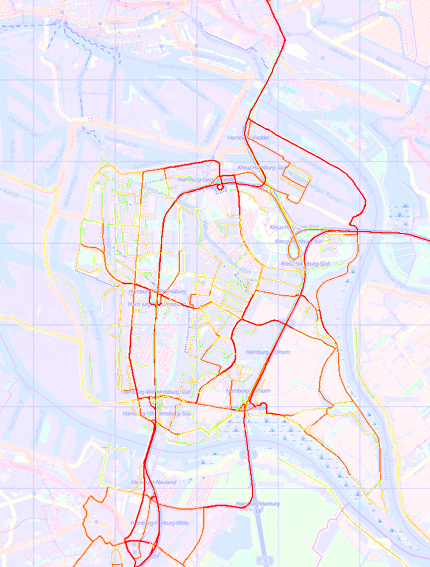
\includegraphics[width=.475\linewidth]{using/figures/b75utilizationold}}%
  {}%
  {}%
  \createsubfigure%
  {}%
  {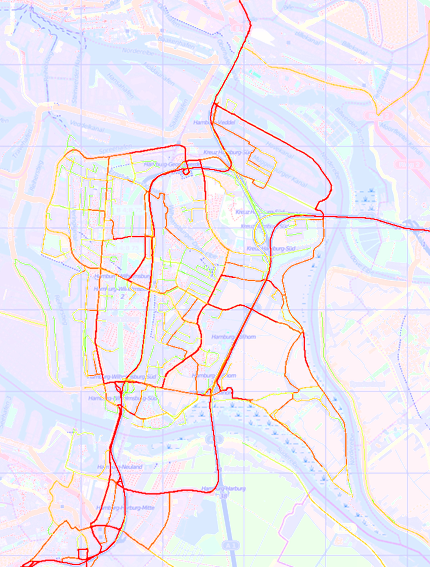
\includegraphics[width=.475\linewidth]{using/figures/b75utilizationnew}}
  {}%
  {}% 
}%
  {}%
% ##################################################################################################################
